\clearpage % clear the prior chapter's page

\chapter{Methodology for rigorous modeling of protein conformational changes by Rosetta using DEER distance restraints}\label{ch:multilateration}
%\vspace{-7mm}
%\bigskip

The contents of this chapter have been previously published \citep*{DelAlamo2021a}.

\bigskip

We describe an approach for integrating distance restraints from \gls{deer} spectroscopy into Rosetta with the purpose of modeling alternative protein conformations from an initial experimental structure. Fundamental to this approach is a multilateration algorithm that harnesses sets of interconnected spin label pairs to identify optimal rotamer ensembles at each residue that fit the \gls{deer} decay in the time domain. Benchmarked relative to data analysis packages, the algorithm yields comparable distance distributions with the advantage that fitting the \gls{deer} decay and rotamer ensemble optimization are coupled. We demonstrate this approach by modeling the protonation-dependent transition of the multidrug transporter PfMATE to an inward facing conformation with a deviation to the experimental structure of less than \SI{2}{\angstrom} $\mathrm{C_{\upalpha}}$ \gls{rmsd}. By decreasing spin label rotamer entropy, this approach engenders more accurate Rosetta models that are also more closely clustered, thus setting the stage for more robust modeling of protein conformational changes.

\section{Introduction}\label{sec:multilateration_main_intro}

Distance measurements between pairs of spin labels by \gls{deer} spectroscopy have been utilized extensively to investigate the structures and dynamics of proteins \citep*{Collauto2017, Evans2020, Kazmier2014, Mishra2014} and the assembly of protein-protein complexes \citep*{Bhatnagar2007, Kim2018, Kim2011, Tessmer2018}. At the fundamental level, \gls{deer} measures magnetic dipolar coupling to infer the distributions of distances between two or more spin labels \citep*{Jeschke2012, Mchaourab2011}. A two-step process typically interprets these distances as spatial restraints describing the protein backbone structure. First, the echo-decay time traces are transformed into distributions consisting of distance components characterized by a mean and width \citep*{FabregasIbanez2020, Hustedt2018, Jeschke2004, Pannier2000, Stein2015}. Second, these distributions are compared to those predicted using one of several strategies, ranging from generic rotamer libraries\citep*{Hagelueken2012, Polyhach2011, Reichel2018}, explicitly modeled pseudoatoms\citep*{Kazmier2014, Raghuraman2014}, or explicitly modeled spin label side chains \citep*{Alexander2013, Dastvan2016, Krug2016, Marinelli2019, Sale2005, Spicher2020}. However, these strategies tend to overestimate the dynamics of flexible probes such as the commonly used \gls{mtssl}. Therefore, the predicted distributions are broad relative to the experimental ones \citep*{Hagelueken2012, Hatmal2012, Islam2013, Jeschke2013, Klose2012}, which hinders \gls{deer}-based evaluation of protein structures or complexes as well as mapping of protein conformational changes. The latter can be obscured entirely if modeled distribution widths exceed distance changes observed between spin labels.1 Another layer of complications in modeling of conformational changes arises if the ensemble of spin label rotamers is allowed to reconfigure, hence providing a low energy pathway to account for changes in distance distributions that originate from backbone movements. Collectively, these caveats limit the accuracy and precision of molecular models generated from \gls{deer} restraints.

Several algorithms have recently been developed to refine ensembles of spin label rotamers by employing multilateration \citep*{Abdullin2015, Gaffney2012, Hagelueken2013, Hays2019, Jeschke2018, Reichel2018}. Multilateration refers to the determination of an object’s position in three-dimensional space given its distance from a constellation of points; common applications include the positioning of electronic devices using the Global Positioning System and of earthquakes epicenters using time-of-arrival data \citep*{Fang1986}.  To utilize this approach to position spin label rotamers requires both a high-resolution starting structure and a set of \gls{deer} distance data consistent with that structure. However, a unique challenge in this endeavor is that spin labels are flexible relative to the protein backbone.  As a result, the ensembles characterizing their positions must be refined simultaneously for all spin labels in a given protein model. 

Molecular dynamics simulations have been used to determine a set of optimized rotamers from explicitly modeled spin labels restrained by experimental distance distributions \citep*{Hustedt2018, Marinelli2015, Marinelli2019, Roux2013}. Alternatively, rotamer libraries have been precomputed and reweighed using either Monte Carlo \citep*{Gaffney2012, Hays2019}, singular value decomposition \citep*{Hagelueken2013}, or nonlinear least-squares minimization \citep*{Jeschke2018}. The positions of these labels can, in turn, be used to more precisely locate paramagnetic ligands or metal ions \citep*{Abdullin2015, Abdullin2021, Gaffney2012, Yang2012} as well as make small-scale refinements to protein structures \citep*{Reichel2018, Wingler2019}. To our knowledge, however, none of these methods have demonstrated that these optimized rotamers can lead to improvements in modeling conformational changes.

Furthermore, these methods generally do not address unique factors confounding multilateration of spin labels. First, the width of a distribution reflects disorder in the solid state as a result of backbone and spin label side chain dynamics at room temperature. Existing multilateration methods generally ignore the former, by assuming the distribution is explained entirely by spin label dynamics \citep*{Gaffney2012, Reichel2018}, or both, by extracting the peak distance from the distribution and discarding the width \citep*{Wingler2019}. Second, relying on distance distributions rather than time domain data propagates assumptions intrinsic to the method used for the transformation of the latter. Depending on the noise level of the experimental measurements, this step can distort true components or introduce ghost components to the distribution. Finally, although \gls{deer} distributions are often reported with confidence bands to reflect the uncertainty inherent to this transformation \citep*{Edwards2016, FabregasIbanez2020, Hustedt2018}, they are generally taken at face value when used for rotamer multilateration. This incorrectly implies that experimental uncertainty is uniformly distributed across the dataset and can lead to rotamers that over- or underfit the \gls{deer} distributions. Collectively, these obstacles prevent the straightforward positioning of spin label ensembles in three-dimensional space and complicate the confidence with which such ensembles can be used for subsequent modeling purposes.

To address these issues, we developed and implemented, as part of the RosettaDEER module, an algorithm that combines rotamer multilateration \citep*{Abdullin2021, Gaffney2012, Jeschke2018} for pairs sharing common spin labeling sites with direct analysis of \gls{deer} time traces. The algorithm calculates a weighted distribution of “pseudo-rotamers”, or inflexible coarse-grained side chains, capable of recapitulating large experimental datasets collected using \gls{deer}. Importantly, this algorithm goes beyond comparable methods by refining these ensembles using raw data in the time domain, rather than distance distributions calculated \emph{a priori}, thus avoiding the loss of information that can occur as result of data transformation. Using experimental collected in the model system T4 Lysozyme and the multidrug transporter PfMATE, we demonstrate that this algorithm is able to fit time domain data as effectively as widely-used \gls{deer} data analysis programs. Integrated with Rosetta, these rotamers ensembles yield substantial improvements in both accuracy and precision of modeling the outward-to-inward isomerization of the multidrug transporter PfMATE, thus reinforcing the notion that coupling analysis of primary data with rotamer optimization is a superior approach for restrained modeling of protein conformational states. 

\section{Results and Discussion}

\subsection{Overview of the multilateration algorithm}

The algorithm capitalizes on the concept of pseudo-rotamers, which are simplified representations of the spin label designed to maximize computational efficiency. A pseudo-rotamer models the spin label side chain as a centroid atom representing the nitroxide ring and its unpaired electron, yielding predicted distance distributions that are comparable to full-atom depictions. Unlike explicit depictions of the spin label used in all-atom simulations, ensembles of pseudo-rotamers do not interact with one another; as a result, the dynamics of spin labels close in space are fully independent. However, in principle, any rotamer library can be used for the multilateration strategy described here \citep*{Alexander2013, Fajer2015, Hagelueken2012, Hatmal2012, Polyhach2011, Spicher2020}.

The transformation of DEER data to distance distributions is an ill-posed mathematical problem necessitating the use of either regularization \citep*{Chiang2005, FabregasIbanez2020, Jeschke2006}, parametric modeling \citep*{FabregasIbanez2020, Hustedt2018, Stein2015}, neural networks \citep*{Worswick2018}, or other methods \citep*{Edwards2016, Pannier2000, Srivastava2016}. Because these methods have intrinsic approximations which could interfere with rotamer ensemble determination, we elected to fit the raw experimental data directly using an iterative simulated annealing strategy that 1) measures all pairwise distances between pseudo-rotamers, 2) converts each distance distribution into a \gls{deer} decay, and 3) calculates the intermolecular dipolar coupling contribution by nonlinear least-squares minimization (Figure \ref{fig:multilateration_main_scheme}). Different levels of noise between \gls{deer} traces linked by multilateration were normalized using estimates obtained from each signal’s corresponding imaginary component \citep*{Marinelli2019}. The algorithm prioritized the generation of parsimonious ensembles by minimizing the total number of pseudo-rotamers with nonzero weights using the \gls{aicc} \citep*{Akaike1973, Sugiura1978}. This metric, which allows for regularization in rotamer space rather than the distance domain, was guided by the heuristic that the flash-freezing process sharpens the distribution of rotamers that contribute to the \gls{deer} signal \citep*{Banham2007, Georgieva2012}. Finally, to account for backbone heterogeneity and the expectation of smoothness in the distance domain, simulated distributions were broadened by a magnitude corresponding to the residues’ intrinsic flexibility, as reported by their respective crystallographic B-factor values \citep*{Sun2019, Yang2007}.

\begin{figure}[h!]
\centering
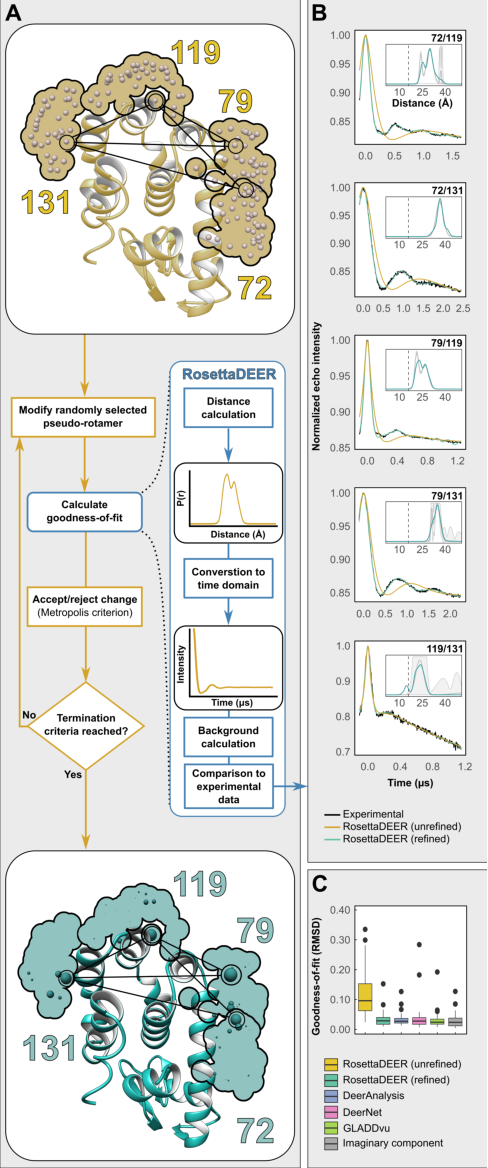
\includegraphics[width=3in]{Figures/multilateration_main_scheme.pdf}
 \caption[Overall scheme of the RosettaDEER multilateration algorithm.]{Scheme of the RosettaDEER multilateration algorithm. (A) Refinement of pseudo-rotamers using the RosettaDEER multilateration algorithm. (B) Representative \gls{deer} traces prior to and following refinement. Insets: Distributions with 95\% confidence bands. (C) Comparison of RosettaDEER to other analysis programs.}
\label{fig:multilateration_main_scheme}
\end{figure}

\subsection{Data analysis benchmark}

We benchmarked this method using experimental DEER data collected in two model proteins, T4 Lysozyme \citep*{Islam2013, Weaver1987} (PDB: 2LZM) and the \gls{mate} transporter PfMATE \citep*{Jagessar2020, Tanaka2013} in its outward-facing conformation (PDB: 6GWH). The extracellular and intracellular spin label pairs of PfMATE were treated independently since they did not share residues in common. These three \gls{deer} datasets consisted of 65 restraints between 47 residues; a subset of the restraints in T4 Lysozyme is shown in \ref{fig:multilateration_main_scheme}.A. We note that unlike the benchmarks used in other multilateration methods, these restraints were highly interconnected; half of the residues were spin labeled in three or more DEER pairs, and in the most extreme case, two residues in T4 Lysozyme were spin labeled across seven pairs (Figure \ref{fig:multilateration_supp_n_restraints}). For each of the three datasets, the RosettaDEER multilateration algorithm was executed for 1000 replicas, with each replica yielding refined pseudo-rotamer ensembles at every spin labeled site.

We compared the resulting fits to those obtained using GLADDvu \citep*{Hustedt2018}, DeerAnalysis \citep*{Jeschke2006}, and DeerNet \citep*{Worswick2018}, which are programs that analyze \gls{deer} data using Gaussian mixture models, Tikhonov regularization, and feed-forward neural networks, respectively. Although other analysis methods are available, we believe these represent a sufficiently diverse range of analytical approaches for the purposes of comparison. We found that the optimum rotamer ensembles, selected by the \gls{aicc}, could recapitulate the experimental \gls{deer} traces as effectively as each of these programs (Figures \ref{fig:multilateration_main_scheme}.B and C, \ref{fig:multilateration_supp_alltraces}, \ref{fig:multilateration_supp_gladdvu}, \ref{fig:multilateration_supp_deeranalysis}, and \ref{fig:multilateration_supp_deernet}). The mean squared errors obtained by the best fit were not statistically different from those obtained by any of these three methods, or from the noise estimated from the imaginary component (Student’s paired one-tailed t-test with Bonferroni correction). However, unlike the latter methods, the interconnectedness of the spin label pairs allowed our algorithm to couple pseudo-rotamer parametrization to the analysis of \gls{deer} data in the time domain.

\begin{wrapfigure}{R}{0.5\textwidth}
\centering
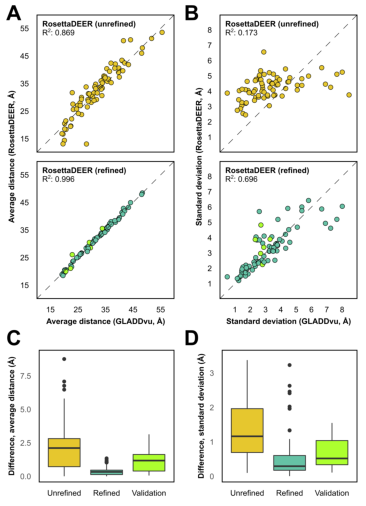
\includegraphics[width=3.25in]{Figures/multilateration_main_fit.pdf}
 \caption[Evaluation of distance distributions by multilateration.]{Evaluation of distance distributions by multilateration. Average distances (A) and widths (B) between pseudo-rotamers prior to (top) and following (bottom) refinement by multilateration. T4 lysozyme distributions omitted from multilateration are shown in light green. (C and D) Boxplots showing the difference between values obtained using GLADDvu and values simulated between pseudo-rotamer ensembles prior to and following refinement.}
\label{fig:multilateration_main_fit}
\end{wrapfigure}

\subsection{Distance distribution benchmark}

We anticipated that the analysis of \gls{deer} data by multilateration would yield distance distributions similar to those obtained using traditional methods. Consistent with this expectation, distributions between refined pseudo-rotamers in both T4L and PfMATE showed remarkable agreement with those obtained using the three methods mentioned above (see insets in Figure \ref{fig:multilateration_main_scheme}.B for examples and  \ref{fig:multilateration_supp_gladdvu}, \ref{fig:multilateration_supp_deeranalysis}, and \ref{fig:multilateration_supp_deernet} for all distributions). For example, the average values of these distributions were within \SI{0.5}{\angstrom} of those obtained using GLADDvu for 60 of the 65 restraints (Figure \ref{fig:multilateration_main_fit}). Additionally, the widths of 52 of these restraints were within \SI{0.5}{\angstrom} of those obtained using GLADDvu. Discrepancies occurred for broad distributions or long distances (because the information content in the time domain is not as well-defined) or components less than \SI{15}{\angstrom} (because these distances minimally contribute to the \gls{deer} signal). Additionally, we uncovered differences when comparing the widths of these distributions to those obtained using DeerAnalysis, likely resulting from small “ghost” side peaks frequently observed in regularization. Discrepancies were also observed when comparing these distributions to those obtained using DeerNet, which yielded widths clustered between \SIrange{2.5}{4.5}{\angstrom} (Figure \ref{fig:multilateration_supp_avgs_stdev}).

Finally, the uncertainty of these distributions was calculated from the five pseudo-rotamer ensembles with the lowest \gls{aicc} values. The resulting confidence bands, which capture 95\% of the variation in the distance distributions, are qualitatively comparable to those obtained using GLADDvu, DeerAnalysis, and DeerNet (Figure \ref{fig:multilateration_supp_conf_bands}).

To further validate the algorithm, we simulated distance distributions for six T4L spin label pairs which were excluded from the multilateration dataset. We observed that the median error between the average distance values fell by 50\% (Figure \ref{fig:multilateration_main_fit}) using the refined rotamers. By contrast, the standard deviations did not significantly sharpen, and their values are similar to those observed prior to refinement. Notably, the uncertainty of these distributions is greater than those of the distributions included in the training set.

\subsection{Conformational change modeling in PfMATE using refined pseudo-rotamers}

While the results above demonstrate the robustness of the multilateration algorithm in identifying optimal spin label pseudo-rotamer ensembles, the central question is whether these provide superior restraint quality for modeling conformational changes. To address this question, we modeled the isomerization of PfMATE between \gls{of} and \gls{if} conformations (shown in Figure \ref{fig:multilateration_main_rmsd}.A and B, respectively), both of which were determined by X-ray crystallography \citep*{Tanaka2013, Zakrzewska2019}. The two conformations differ primarily in the relative orientations of the N- and C-terminal domains resulting from changes in the backbone dihedral angles of \gls{tmh}7. Of direct relevance to the question addressed here, distance distributions between pairs of spin labels measured at pH 7.5 and pH 4.0 were shown to be consistent with the OF and IF conformations, respectively \citep*{Jagessar2020}.



We generated several thousand models, using Rosetta \citep*{Leaver-fay2011, Leman2020} without \gls{deer} restraints, by perturbing \gls{tmh}7 and found that none of the built-in membrane protein scoring functions \citep*{Alford2020, Alford2015, Weinstein2019, Yarov-Yarovoy2006} could identify the \gls{if} state by score alone (Figure \ref{fig:multilateration_supp_scores}) even if it was included in the initial model set. Thus, from an \gls{mc} modeling perspective, the \gls{of}-to-\gls{if} conformational transition can be sampled, but not necessarily identified, without experimental data.

\begin{table}[h!]
\scriptsize
%\renewcommand{\tabcolsep}{0.09cm}
\renewcommand{\tabcolsep}{0.15cm}
\centering
\caption[Restraints used to score PfMATE models.]{Restraints used to score PfMATE models.}

\newcolumntype{Y}{>{\raggedright\arraybackslash}X}

\begin{center}
\begin{tabular}{l l l l l l l l l l l}
\toprule \\
\textbf{Set} &	\textbf{1} &	\textbf{2} &	\textbf{3} &	\textbf{4} &	\textbf{5} &	\textbf{6} &	\textbf{7} &	\textbf{8} &	\textbf{9} &	\textbf{10} \\
\midrule \\
1 &	120/269 &	215/318 &	120/413 &	215/394 &	134/269 &	215/442 &	186/269 &	240/318 &	186/348 &	240/442 \\
2 &	120/413 &	215/318 &	134/269 &	215/394 &	186/348 &	215/442 &	186/269 &	240/318 &	196/348 &	240/442 \\
3 &	240/442 &	186/348 &	215/394 &	196/348 &	215/442 &	120/269 &	215/318 &	186/269 &	240/318 &	120/413 \\
4 &	215/318 &	186/269 &	240/442 &	120/413 &	240/318 &	134/269 &	186/348 &	196/348 &	215/442 &	120/269 \\
\bottomrule \\
\end{tabular} 
\end{center}




\label{tab:pfmate_restraints}
\end{table}

\begin{wrapfigure}{r}{0.5\textwidth}
\centering
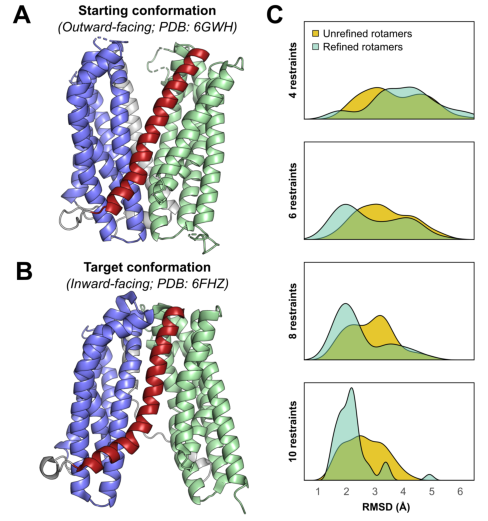
\includegraphics[width=3.25in]{Figures/multilateration_main_rmsd.pdf}
 \caption[Modeling conformational changes in the multidrug transporter PfMATE.]{Modeling conformational changes in the multidrug transporter PfMATE. (A) \Gls{of} and (B) \gls{if} crystal structures of PfMATE. N- and C-terminal domains shown in purple and green, respectively, with \gls{tmh}7 in red. (C) \Gls{rmsd} values of ten best-scoring models relative to the \gls{if} conformation using pseudo-rotamers either refined by multilateration (teal) or available by default (yellow).}
\label{fig:multilateration_main_rmsd}
\end{wrapfigure}

To test the notion that \gls{deer} restraints interpreted with the refined pseudo-rotamers can drive convergence of Rosetta modeling, we identified spin label pairs where the \gls{epr} lineshape showed minimal changes upon a pH shift from 7.5 to 4.0, supporting the approximation that the spin label rotamer ensembles are invariant and thus were not allowed to reconfigure during Rosetta modeling (Table \ref{tab:pfmate_restraints}). From these pairs, 40 sets of restraints were generated, each of which consisted of one to ten spin label pairs. Using scoring functions to assess the agreement with the DEER restraints (see section \ref{sec:multilateration_main_methods}), the \gls{of}-to-\gls{if} conformational transition was modeled by perturbing the dihedral angles of \gls{tmh}7. \Gls{deer} distributions were simulated using either the pseudo-rotamers ensembles refined by multilateration or the unrefined ensembles available to RosettaDEER by default. Agreement with the experimental distributions was evaluated by the overlap between the experimental and simulated distance distributions. Similarity to the inward-facing crystal structure was quantified by the \gls{rmsd} of the alpha carbons excluding \gls{tmh}s 1 and 7.


We observed a striking contrast between the effectiveness of the refined and unrefined ensembles (Figure \ref{fig:multilateration_main_rmsd}.C). The default rotamer library did not effectively improve the average \gls{rmsd} values of the ten lowest-scoring models beyond \SIrange{2.0}{3.5}{\angstrom}. By contrast, the use of multilaterated pseudo-rotamers converged upon inward-facing models to \SIrange{1.5}{2.5}{\angstrom} $\mathrm{C_{\upalpha}}$ \gls{rmsd} using restraints obtained from the same spin label pairs.

Alongside these improvements in accuracy, the sharper range of \gls{rmsd} values suggested that multilateration improved model precision. Distributions of representative distances in the intracellular and extracellular sides of the top ten models (Figures \ref{fig:multilateration_main_convergence}.A and B) revealed that, when using the default pseudo-rotamers, a majority of these models failed to close the extracellular cavity and were less inward-open than the \gls{of} structure (Figure \ref{fig:multilateration_main_convergence}.C), even when ten restraints were used. By contrast, models obtained using refined pseudo-rotamers deviated less drastically from the crystal structure. Nonetheless, these models were virtually all less inward-open than the crystal structure, consistent with shorter-than-expected experimental \gls{deer} measurements on the intracellular side at pH 4.0 (Figure \ref{fig:multilateration_main_convergence}.D) \citep*{Jagessar2020} .


\subsection{Concluding remarks}

Our results highlight a strategy to improve the quality of models obtained from \gls{epr} restraints. We envision that the main application of this strategy is to model alternate conformational states starting from an experimental structure and a set of interconnected \gls{deer} data. By implementing this algorithm in Rosetta, we hope to encourage its use for a wide variety of modeling applications, such as protein-protein docking and \emph{de novo} folding. Moreover, further development of this approach, as well as extensive use of multilateration in the design of spin label pairs, will open the door to modeling proteins where conformational changes are defined by more complex modes of motion.

\section{Materials and Methods}\label{sec:multilateration_main_methods}

\subsection{Overview of the model-based approach}


\begin{wrapfigure}{r}{0.6\textwidth}
\centering
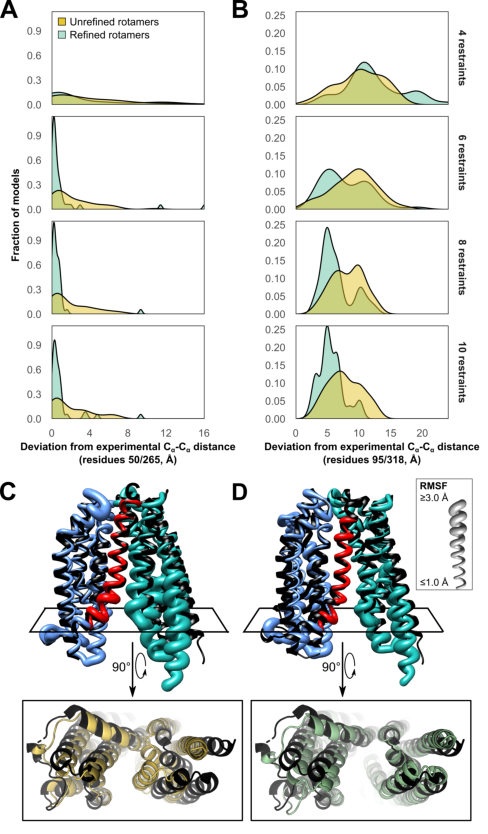
\includegraphics[width=3.25in]{Figures/multilateration_main_convergence.pdf}
 \caption[Models obtained using multilaterated rotamers more closely resemble the IF structure.]{Models obtained using multilaterated rotamers more closely resemble the IF structure. Deviation between experimental and predicted $\mathrm{C_{\upalpha}}$-$\mathrm{C_{\upalpha}}$ distances observed between pairs on the A) extracellular and B) intracellular sides. Models obtained using ten restraints either with C) default or D) refined rotamers (\gls{if} structure in black).}
\label{fig:multilateration_main_convergence}
\end{wrapfigure}

The objective of the RosettaDEER multilateration algorithm is to fit a set of \gls{deer} data by weighting the nitroxide pseudo-rotamers available to each spin-labeled residue in a protein structural model. Each replicate of the algorithm independently generates a unique set of pseudo-rotamer ensembles for each spin-labeled residue. For clarity throughout this text, we will refer to these outputs as "coordinate models", to differentiate them from the starting structural models. The space accessible to the unpaired electron of each residue’s spin label is divided into fifty discrete pseudo-rotamers, which are shown as small spheres in Figure \ref{fig:multilateration_main_scheme}.A. RosettaDEER then identifies and removes pseudo-rotamers that clash with the protein backbone. Each residue’s ensemble of pseudo-rotamers represents a probability density function of the space accessible to the unpaired electron of that residue’s spin label. As a result, following refinement using this algorithm, the weights of a coordinate model’s pseudo-rotamers for any given residue are tightly coupled to those of other residues.



In this study we focus our attention on coordinate models with high parsimony. For example, coordinate models capable of recapitulating \gls{deer} traces using only one pseudo-rotamer per residue are prioritized over those with two or more. However, if the \gls{deer} trace indicates a broad and multimodal distribution, additional pseudo-rotamers may be necessary to improve the goodness-of-fit. The total number would ideally be no greater than the minimum required to fit the data, and multiple combinations of pseudo-rotamers may be equally consistent with the data. We identified parsimonious coordinate models using the \gls{aicc} \citep*{Akaike1973, Burnham2002, Sugiura1978}:

\begin{equation}
AICc = -2 * \ln(L(\hat{\vartheta}|D)
\label{eq:aicc}
\end{equation}

This metric balances two competing objectives of 1) fitting the experimental data as well as possible and 2) simplifying the model as much as possible. The leftmost term, goodness-of-fit, is expressed as the maximum likelihood estimate of the coordinate model with parameters $\vartheta$ given the experimental \gls{deer} data $D$ and is described below. The middle and rightmost term express the complexity of the model, with the variable $K$ corresponding to the total number of parameters in the coordinate model and $n_{\mathup{total}}$ corresponding to the total number of time points in the experimental \gls{deer} data. $K$ includes the number of pseudo-rotamers with nonzero weights, as well as the number of parameters required to fit the intramolecular \gls{deer} data in the time domain. The rightmost term, which converges to zero as the data-to-parameter ratio increases, serves as further regularization in modeling cases where less experimental data is available (in this case corresponding to the number of time points in all \gls{deer} traces). Overall, the \gls{aicc} quantifies the expectation that few spin label rotamers contribute to the distance distribution.

\subsection{Detailed description of the multilateration algorithm}

The multilateration algorithm is implemented in Rosetta \citep*{Leaver-fay2011, Leman2020} as part of the RosettaDEER package and can be run using RosettaScripts \citep*{Fleishman2011}. It uses an iterative simulated annealing approach and is therefore non-deterministic. As a result, it obtains diverse sets of solutions when executed multiple times. However, there is no guarantee that the global minimum solution is obtained using this algorithm.

The positions of the pseudo-rotamers are kept fixed in space throughout the duration of the algorithm, e.g., they are reweighted, rather than moved. Initial positions are obtained from the nitroxide bond midpoints of each rotamer in the Rosetta \gls{mtssl} rotamer library following clash evaluation \citep*{Alexander2013}. At the start of the algorithm, one of these pseudo-rotamers is randomly chosen for each residue and has its weight set to 1; the rest have weights set to zero.

The algorithm then proceeds as follows:

\begin{itemize}
    \item The weight of a randomly chosen pseudorotamer is modified by a randomly chosen number. Initially this value ranges uniformly from -0.1 to 0.1.
    \item The weight change is applied, and the resulting sum-of-squared residuals is calculated as discussed below.
    \item Any move that decreases the sum-of-squared residuals is accepted, while any move that increases it is accepted with the following probability (with $\mathup{iter}$ being the current iteration):
    \begin{equation}
        p_{accept}= \exp \left( - \frac{\ln \left( L \left( \vartheta_{\mathup{iter+1}} | D \right) \right) - \ln \left( L \left( \vartheta_{\mathup{iter}} | D \right) \right) }{k_{\mathup{B}}T} \right)
        \label{eq:multilateration_accept}
    \end{equation}
    \item The Boltzmann temperature $k_{\mathup{B}}T$ starts at 1.5 and asymptotically approaches zero with each iteration as the algorithm proceeds. A total of 2500 trials per round are performed per \gls{deer} trace in the dataset. However, each round is aborted if 500 consecutive trials fail to sample an improvement.
    \item At the end of each round, the temperature $k_{\mathup{B}}T$ is raised to 1.5. If no improvements were sampled, the magnitude of the weight changes made to coordinates is reduced by a factor of $\sqrt{10}$. Once this magnitude reaches $10^{−4}$, the algorithm is concluded.
\end{itemize}

For PfMATE, we used a non-three-dimensional background model to fit the intermolecular contribution of the experimental signal. This required a modification to the algorithm in which the first round of optimization was performed using a three-dimensional background. The first time $k_{\mathup{B}}T$ was reset to 1.5, this restriction was removed. Otherwise, the dimensionality of the intermolecular background coupling was found to immediately drop to a value of 2, trapping the solution in a local minimum.

\subsection{Simulation of DEER distance distributions}

To simulate distance distributions between two spin-labeled residues u and v, pairwise distances were measured between all coordinates belonging to each residue. To account for backbone heterogeneity, each of these measurements were then broadened by a value equal to the pairwise \gls{rmsf} as inferred from the crystallographic isotropic B-factor of the residues’ $\mathrm{C_{\upalpha}}$ atoms:

\begin{equation}
    RMSF_{\mathup{u}}=\sqrt{\frac{3 B_{\mathup{u}, C_{\upalpha}}}{8 \pi^{2}}}
\end{equation}

\begin{equation}
    RMSF_{\mathup{uv}}=\sqrt{RMSF_{\mathup{u}}^{2}+RMSF_{\mathup{v}}^{2}}
\end{equation}

The result is equivalent to the convolution of the original distribution with a Gaussian distribution with a width of $RMSF_{\mathup{uv}}$. Regions of proteins with higher B-factors, such as loops, have previously been found to exhibit a greater degree of backbone flexibility in solution \citep*{Billeter1992, Powers1993, Yang2007}. Failure to account for backbone flexibility could potentially overstate the intrinsic dynamics of the spin label and decrease the precision of the models generated using the pseudo-rotamers obtained this way. We did not normalize the experimental B-factors to account for differences in experimental crystallographic resolution, since such differences may reflect variations in the backbone disorder of different proteins.

\subsection{Evaluating coordinate models obtained from raw DEER traces}

The data $D$ consist of $N$ decay traces ($V_{\mathup{exp}}$), e.g., $D = {V_{\mathup{exp,1}}, V_{\mathup{exp,2}},…, V_{\mathup{exp,N}}}$, with the $\mathup{i}$th decay trace consisting of $n_{\mathup{i}}$ time points for a total of $n_{\mathup{total}}$ experimental time points among all experimental traces. In this case, the likelihood of the model was evaluated by the noise-normalized sum-of-squared residuals to the experimental data:

\begin{equation}
    \ln \left( L \left( \vartheta | D \right) \right)=-\frac{ n_{\mathup{total}}}{2} * \ln \left( \frac{1} {n_{\mathup{total}}} \sum_{\mathup{i}=1}^{N} \sum_{\mathup{i}_{t}}^{n_{\mathup{i}}} \left( \frac{ V_{\mathup{exp,i}} \left( t_{\mathup{i_t}} \right) - V_{\mathup{intra,i}} \left( t_{\mathup{i_{t}}} | \vartheta \right) }{\sigma_{\mathup{i}}} \right)^2 \right)
    \label{eq:multilateration_loglikelihood}
\end{equation}

Here $\sigma_{\mathup{i}}$ is the standard deviation of the noise corresponding to the $\mathup{i}$th decay trace, $V_{\mathup{exp,i}}\left(t_{\mathup{i}} \right)$ refers to the experimental data at the $i_{\mathup{t}}$th time point of decay trace $\mathup{i}$, and $V_{\mathup{intra,i}}\left( t_{\mathup{i}_{t}}|\vartheta \right)$ refers to the value of the simulated data in decay trace $\mathup{i}$ at time point it given the model parameters $\vartheta$. The values of $\sigma_{\mathup{i}}$ were calculated from the imaginary component of each \gls{deer} trace. Normalizing the data to the noise was necessary to satisfy the assumption that the sum of squared residuals is independently and identically distributed. Forgoing this correction led to overfitting of noisier \gls{deer} traces and underfitting of less noisy traces.

Simulation of DEER traces occurred in three steps. First, the distance distributions were obtained from the model coordinates as described above. Second, the intramolecular form factor was calculated for each time point $t_{\mathup{i_t}}$:

\begin{equation}
    V_{\mathup{intra,t}}\left( t_{\mathup{i_{t}}} | \vartheta \right) = \sum_{\mathup{j}=1}^{m} P_{\mathup{sim,i}} \left( r_{\mathup{j}} | \vartheta \right) \int_{0}^{\frac{\pi}{2}} \sin \left( \theta \right) * \cos \left( \frac{ \left( 1 - 3 \cos^{2} \theta \right) \mu_{0} \mu_{\mathup{B}}^2 g^2 t_{\mathup{i_{t}}} }{4 \pi \hslash r_{\mathup{j}}^{3}} \right) \mathup{d} \theta
    \label{eq:multilateration_kernel}
\end{equation}

Here, $g$ is the electron g-factor, $\mu_{\mathup{0}}$ is the vacuum permeability constant, $\mu_{\mathup{B}}$ is the Bohr magneton, $t_{\mathup{i}_{t}}$ is the $i_{\mathup{t}}$th time point in microseconds, $r$ is the bin distance in nanometers, and $\theta$ is the angle between the bulk magnetic field and the interspin vector.

In the third step, the modulation depth, background slope, and dimensionality (in the case of PfMATE) were determined using nonlinear least-squares minimization. This background was modeled using the stretched exponential function $B \left( t \right) = exp \left( - \left( kt \right)^\frac{d}{3} \right)$, where $d$ refers to the dimensionality of the background coupling and was constrained to 3.0 for T4 Lysozyme and to between 2.0 and 3.5 for PfMATE. In the latter case, we generally obtained values ranging from 2.0 to 2.5. These parameters were determined using an initial search as previously described and were fine-tuned throughout the duration of the algorithm using the Levenberg-Marquardt algorithm.

\subsection{Determination of distance distributions}

We used GLADDvu \citep*{Hustedt2018} and DeerAnalysis2019b \citep*{Jeschke2006} to fit the data and obtain distance distributions. Each \gls{deer} trace was truncated by \SI{500}{ns} to avoid fitting artifacts. Sum-of-Gaussian distributions were obtained with GLADDvu using the interior point method. The distribution with the lowest Bayesian Information Criterion was selected. Distributions were also obtained using Tikhonov regularization with an L-curve criterion with default settings, as well as the generic DeerNet neural network ensemble, using DeerAnalysis2019b. Confidence bands and/or error margins were obtained using the delta method for GLADDvu, the Validation tool for Tikhonov regularization, and built-in ensemble statistics for DeerNet.

\subsection{Application to T4 Lysozyme and PfMATE}

The algorithm as described above was applied to T4 Lysozyme (PDB: 2LZM) and \gls{of} PfMATE structure (PDB: 6GWH). For PfMATE, the data were further separated into the extracellular restraints and the intracellular restraints. The algorithm was executed one thousand times for each of these three datasets. Each of the one thousand coordinate models were scored using the \gls{aicc} (Equation \ref{eq:aicc}).

\subsection{Modeling the OF-to-IF conformational change of PfMATE}

Modeling the outward-to-inward conformational change of PfMATE was achieved using an \gls{mc} fragment insertion approach implemented in RosettaScripts. This protocol randomly changes the backbone dihedral angles of certain residues chosen at random to match those of a similar stretch of residues found in protein structures deposited in the PDB. Only residues 1–50 and 241–268 were perturbed. Peptide fragments were obtained from a July 2011 version of the PDB using the Robetta web server \citep*{Kim2011} with homologous protein structures removed. The fragment insertion protocol was executed 1000 times in RosettaScripts using the \emph{score3} scoring function and was repeated for 5000 cycles. The Boltzmann temperature was set to 1.0. The following scoring function was then used to quantify the similarity between the experimental and simulated DEER distributions:

\begin{equation}
    S_{\mathup{DEER}} = \sum_{\mathup{i}=1}^{N} \ln \left( \sum_{\mathup{j}=1} p_{\mathup{sim,ij}}p_{\mathup{exp,ij}} \right)
\end{equation}

In the event that an experimental and simulated distribution did not overlap, the inner term resolves to $\ln \left(0 \right)$. Under these circumstances, this value was automatically set to -87.0, which is equivalent to the natural logarithm of the lowest non-negative value that can be described by a single-precision floating point number. The choice of this scoring function is discussed in Appendix \ref{app:scoring}.

\section{Acknowledgements}

We thank Dr. Derek P. Claxton and Dr. Richard A. Stein for critical reading of the manuscript, and Dr. Eric Hustedt for both fruitful discussions regarding the \gls{aicc} and model-based fitting as well as critical reading of the manuscript.